
\begin{question}
Please make a frequency histogram from the following (unsorted)
continuous data by rounding to the nearest integer.

\begin{longtable}[]{@{}rrrrrr@{}}
\toprule
32.8201 & 27.7238 & 26.8074 & 29.1022 & 26.8669 & 31.1417\tabularnewline
27.2485 & 29.5684 & 32.2030 & 28.2653 & 27.0917 & 31.5793\tabularnewline
29.1215 & 27.6318 & 27.4419 & 29.8927 & 32.5300 & 26.7177\tabularnewline
30.3773 & 31.1362 & 30.5521 & 30.5156 & 31.8444 & 31.9692\tabularnewline
30.1981 & 31.9197 & 31.0182 & 31.5077 & 30.5075 & 28.5467\tabularnewline
\bottomrule
\end{longtable}
\end{question}

\begin{solution}
Make a frequency table.

\begin{longtable}[]{@{}rr@{}}
\toprule
value & frequency\tabularnewline
\midrule
\endhead
27 & 6\tabularnewline
28 & 3\tabularnewline
29 & 3\tabularnewline
30 & 4\tabularnewline
31 & 6\tabularnewline
32 & 6\tabularnewline
33 & 2\tabularnewline
\bottomrule
\end{longtable}

Make the histogram.

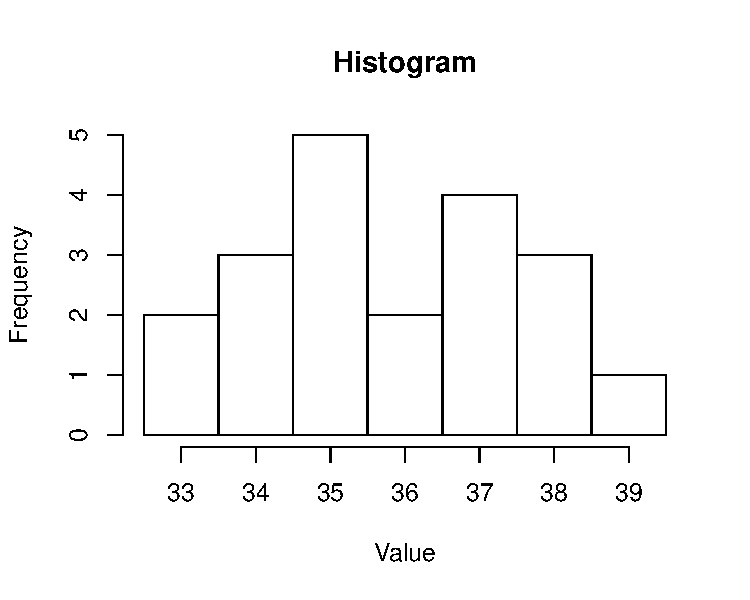
\includegraphics{barchart-1.pdf}\\
\end{solution}

